% !TEX root = main.tex
\chapter{Simulações e Resultados}
\label{cha:results}


\begin{figure}[H]
    \centering
    \subfigure[Época 0]
    {
        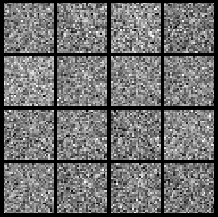
\includegraphics[width=0.30\textwidth]{figs/MNIST/new_tests/_epoch_0_batch_0.png}
        \label{fig:results_mnist_epoch-0}
    }
    \hspace{0.5cm}
    \subfigure[Época 3]
    {
        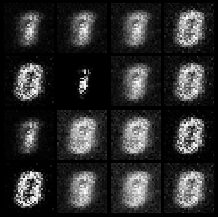
\includegraphics[width=0.30\textwidth]{figs/MNIST/new_tests/_epoch_3_batch_500.png}
        \label{fig:results_mnist_epoch-3}
    }
    \\
    \vspace{0.5cm}
    \subfigure[Época 32]
    {
        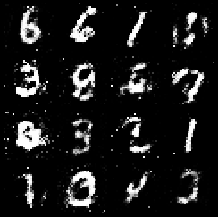
\includegraphics[width=0.30\textwidth]{figs/MNIST/new_tests/_epoch_32_batch_400.png}
        \label{fig:results_mnist_epoch-32}
    }
    \hspace{0.5cm}
    \subfigure[Época 299]
    {
        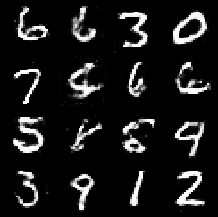
\includegraphics[width=0.30\textwidth]{figs/MNIST/new_tests/_epoch_299_batch_500.png}
        \label{fig:results_mnist_epoch-299}
    }
    \caption{Gerações da GAN \textit{Vanilla} para o \textit{dataset} MNIST em diferentes épocas.}
    \label{fig:results_mnist}
\end{figure}



\pagebreak
\newpage



\begin{figure}[H]
    \centering
    \subfigure[Erros.]
    {
        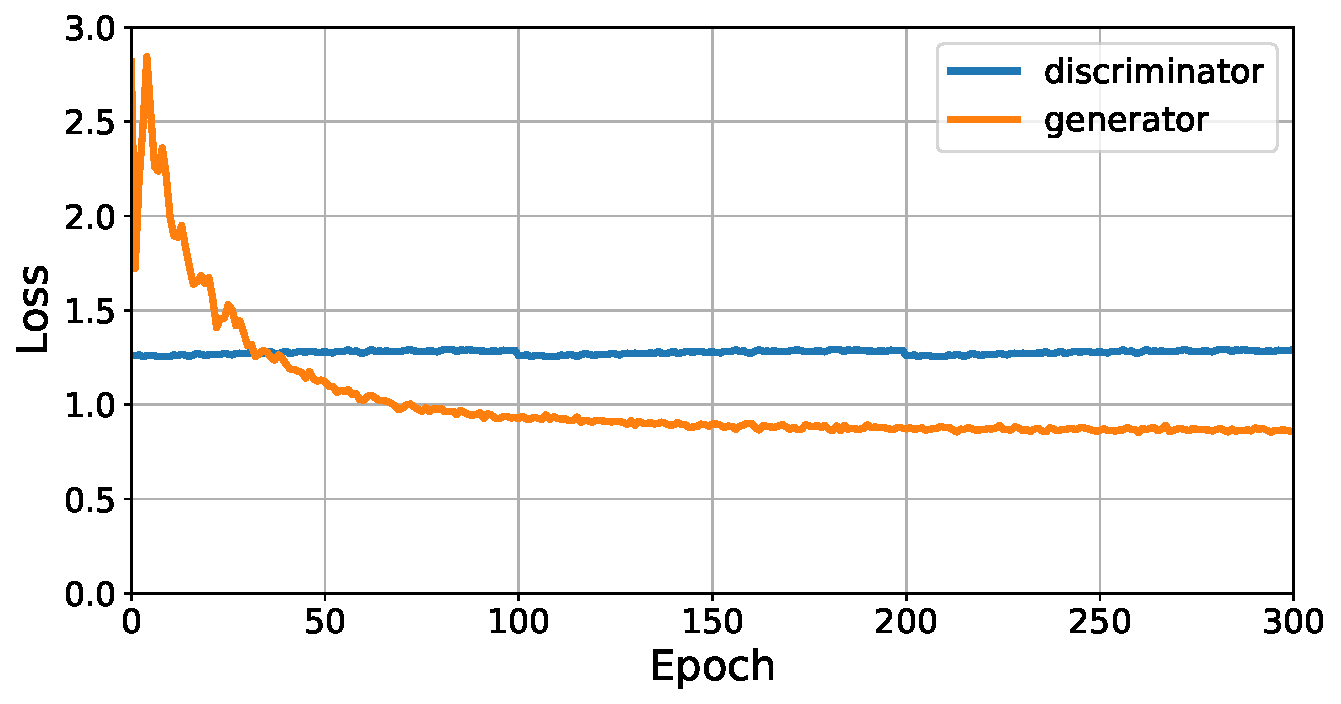
\includegraphics[width=0.75\textwidth]{figs/results/pytorch_vanilla_mnist_loss_0-299.pdf}
        \label{fig:results_pytorch_vanilla_mnist_loss}
    }
    \\
    \vspace{0.5cm}
    \subfigure[Incertezas.]
    {
        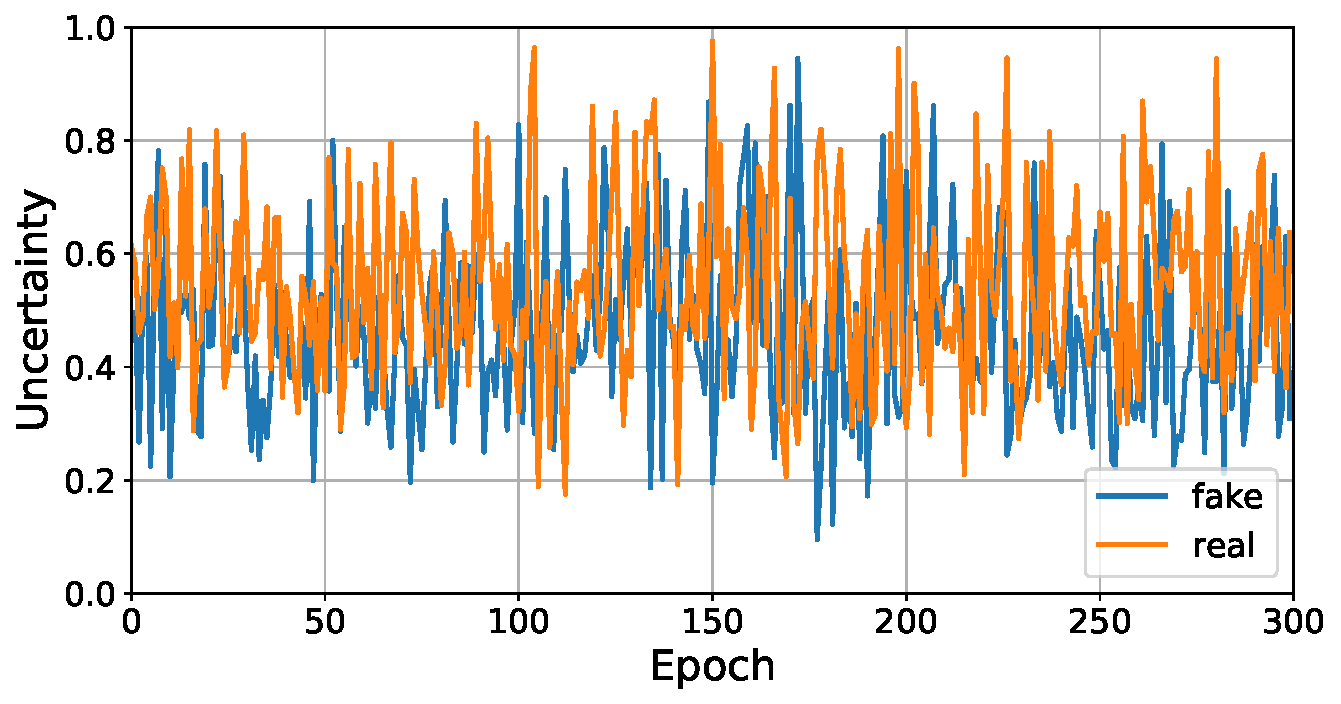
\includegraphics[width=0.75\textwidth]{figs/results/pytorch_vanilla_mnist_uncertainty_0-299.pdf}
        \label{fig:results_pytorch_vanilla_mnist_uncertainty}
    }
    \caption{Erros e incertezas da GAN \textit{Vanilla} para o \textit{dataset} MNIST em diferentes épocas.}
    \label{fig:results_pytorch_vanilla_mnist_scores}
\end{figure}